\documentclass[12pt, letterpaper, titlepage]{article}

\usepackage{amsmath}
\usepackage{booktabs}
\usepackage{amsthm}
\usepackage{graphicx}
\usepackage[margin=1in]{geometry}
\usepackage{hyperref}
\hypersetup{colorlinks = true, linkcolor = blue, citecolor=blue, urlcolor = blue}
\usepackage{natbib}
\usepackage{enumitem}
\usepackage{setspace}
\usepackage{lipsum}

\usepackage[pagewise]{lineno}
%\linenumbers*[1]
% %% patches to make lineno work better with amsmath
\newcommand*\patchAmsMathEnvironmentForLineno[1]{%
 \expandafter\let\csname old#1\expandafter\endcsname\csname #1\endcsname
 \expandafter\let\csname oldend#1\expandafter\endcsname\csname end#1\endcsname
 \renewenvironment{#1}%
 {\linenomath\csname old#1\endcsname}%
 {\csname oldend#1\endcsname\endlinenomath}}%
\newcommand*\patchBothAmsMathEnvironmentsForLineno[1]{%
 \patchAmsMathEnvironmentForLineno{#1}%
 \patchAmsMathEnvironmentForLineno{#1*}}%

\AtBeginDocument{%
 \patchBothAmsMathEnvironmentsForLineno{equation}%
 \patchBothAmsMathEnvironmentsForLineno{align}%
 \patchBothAmsMathEnvironmentsForLineno{flalign}%
 \patchBothAmsMathEnvironmentsForLineno{alignat}%
 \patchBothAmsMathEnvironmentsForLineno{gather}%
 \patchBothAmsMathEnvironmentsForLineno{multline}%
}

% control floats
\renewcommand\floatpagefraction{.9}
\renewcommand\topfraction{.9}
\renewcommand\bottomfraction{.9}
\renewcommand\textfraction{.1}
\setcounter{totalnumber}{50}
\setcounter{topnumber}{50}
\setcounter{bottomnumber}{50}

\newcommand{\jy}[1]{\textcolor{blue}{JY: #1}}
\newcommand{\eds}[1]{\textcolor{red}{EDS: (#1)}}


\title{Title}

\author{Michael Zheng\\
%   \href{mailto:anthony.zeimbekakis@uconn.edu}
% {\nolinkurl{anthony.zeimbekakis@uconn.edu}}\\
  Elizabeth Schifano\\
  Jun Yan\\[1ex]
  Department of Statistics, University of Connecticut\\
}
\date{}

\begin{document}
\maketitle

\doublespace

\begin{abstract}
\lipsum[1]
Text

\bigskip
\noindent\sc{Keywords}:
KEYWORD;
KEYWORD;
\end{abstract}

\section{Introduction}
\label{sec:intro}
\lipsum[1]

% one equation in displaystyle %
\begin{equation}
  \label{eq:eq1}
  D = F(x) - F_{\hat\theta_n}(x) |.
\end{equation}

\section{Unspecified Parameters}
\label{sec:fitted}

\lipsum[1]

% one in-line math expression %
$B_{n}(x) = \sqrt{n}(F_{n}(x) - F_{\hat\theta_n}(x))$

\section{Serially Dependent Data}
\label{sec:dependence}

\lipsum[1]

% one table %
\begin{center}
\begin{tabular}{ |c|c|c| } 
 \hline
 cell1 & cell2 & cell3 \\ 
 cell4 & cell5 & cell6 \\ 
 cell7 & cell8 & cell9 \\ 
 \hline
\end{tabular}
\label{table:table1}
\end{center}

\section{Unspecified Parameters and Serially Dependent Data}
\label{sec:fittedwithdependence}

\lipsum[1]

% one figure %
I would prefer that \autoref{fig:example} be placed right after this paragraph.
If that is not possible, I would like it at the the top of a page.

\begin{figure}[ht]
  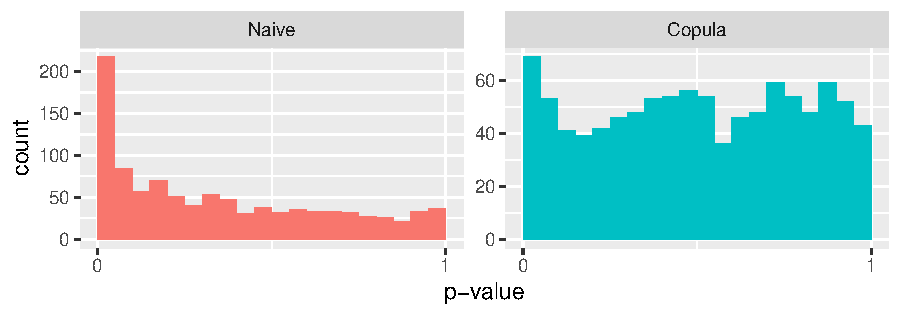
\includegraphics[width=\textwidth]{hist_ar1_D}
  \caption{Caption}
  \label{fig:example}
\end{figure}

\section{Conclusion}
\label{sec:conclusion}

% parenthetical citation %
A copula is a
multivariate distribution with standard uniform marginal distributions, which
completely characterizes the dependence structure of a multivariate
distribution \citep{Copula, Hofert}

% citation within the text %
For example, \citet{Noether} demonstrated the conservativeness of
the KS test when applied to discontinuous distributions.

% cross referencing sections using \label and \ref %
As mentioned in section \ref{sec:intro}, different elements can be referenced within a document.

% cross referencing figures using \label and \ref %
As mentioned in section \ref{fig:example}, different elements can be referenced within a document.

% cross referencing tables using \label and \ref %
As mentioned in section \ref{table:table1}, different elements can be referenced within a document.

\bibliographystyle{chicago}
\bibliography{citations.bib}


\end{document}
